\documentclass{article}
\usepackage{graphicx}
\oddsidemargin 0.25in \evensidemargin 0.25in
\topmargin -0.5in
\textwidth 6.5in \textheight 9in
\headheight 0.18in \footskip 0.16in
\leftmargin -0.5in \rightmargin -0.5in

\newcommand{\sym}[1]{\hspace*{\fill}($#1$)}

\begin{document}

\noindent{\LARGE \textbf{Mutual Inductor}
\hspace{\fill}\textbf{K}}\\
\normalsize
\newline
\rule{\textwidth}{0.5mm}

\normalsize
\begin{figure}[h]
\centerline{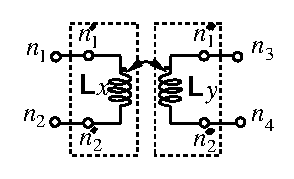
\includegraphics[width=2in]{k_spice.ps}} \caption{K --- Mutual
inductor element.}
\end{figure}


\noindent\rule{\textwidth}{0.5mm}
\newline
\texttt{SPICE} \textit{Form:}
\newline
{\tt K}{\it name} {\tt L}{\it name1} {\tt L}{\it name2} {\it
CouplingValue}
\newline

\begin{tabular}{r l}
{\tt L}{\it name1} & is the name of the first inductor of the\\
& coupled inductor list. The first node of {\tt L}{\it name1} is\\
& dotted using the dot convention. In the mutual coupled
inductor\\
& model (the default model) the value of {\tt L}{\it name1} is
the\\
& self inductance $L_1$. In the transformer {\tt CORE} model\\
& (which is used if a {\it ModelName} is supplied) the value of\\
& {\tt L}{\it name1} is the number of turns $N_1$.\\
& (Required)\\
{\tt L}{\it name2} & is the name of the second inductor in the\\
& coupled inductor list. The first node of {\tt L}{\it name2} is\\
& dotted using the dot convention. In the mutual coupled
inductor\\
& model the value of {\tt L}{\it name2} is the self inductance\\
& $L_2$. In the transformer {\tt CORE} model (which is used if a\\
& {\it ModelName} is supplied the value of {\tt L}{\it name2} is\\
& the number of turns $N_2$.\\
& ( Required.)\\
{\tt L}{\it nameN} & is the name of $N$th inductor in the
coupled\\
& inductor list. The first node of {\tt L}{\it nameN} is dotted\\
& using the dot convention. In the mutual inductor model the
value\\
& of {\tt L}{\it nameN} is the self inductance $L_N$. In the\\
& transformer {\tt CORE} model (which is used if a {\it
ModelName})\\
& is supplied the value of {\tt L}{\it name2} is the number of\\
& turns $N_N$. \\
&  for $N > 2$.\\
{\it CouplingValue} & is the coefficient of mutual coupling of
the inductors.\\
& (Units: none; Required; Symbol: $K_{\mathrm{COUPLING}}$; $ 0 <
K_{\mathrm{COUPLING}} \le 1$)\\
{\it ModelName} & is the optional model name.\\
{\it Size} & is the size scaling factor. It scales the magnetic\\
& cross-section and represents the number of lamination layers.\\
               & (Units: none; Optional; Default: 1; Symbol: $Size$)
\end{tabular}
\newline
\rule{\textwidth}{0.5mm}
\newline
\textit{Example:}
\newline
\texttt{K43 LAA LBB 0.999 \\ KXFRMR L1 L2 0.87}
\newline
\rule{\textwidth}{0.5mm}
\newline
\textit{Description:}\\
Model Type {IND}: The mutual coupled inductor
model represents coupled inductors by self inductances $L_i$ and
mutual inductances $M_{ij}$. This is the model used if a
{\tt CORE model} is not supplied. Here $L_i$ is the self
inductance of the $i$th inductor element and $M_{ij}$ is the
mutual inductance of the $i$th and $j$th inductor elements. The
mathematical model of the coupled element consists of voltage
sources controlled by the time derivatives of current. If two
inductors are coupled
\begin{equation}
      V_1 = L_1 {{\textstyle dI_1} \over {\textstyle dt}}
         + M_{12} + {{\textstyle dI_2} \over {\textstyle dt}}
\end{equation}
and
\begin{equation}
      V_2 = L_2 {{\textstyle dI_2} \over {\textstyle dt}}
         + M_{21} + {{\textstyle dI_1} \over {\textstyle dt}}
\end{equation}
If $N$ inductors are coupled the mathematical model is
\begin{equation}
      V_i = L_i {{\textstyle dI_i} \over {\textstyle dt}}
         + \sum_{\shortstack{$j=1$\\ $j\ne i$}}^N
         M_{ij} {{\textstyle dI_j} \over {\textstyle dt}}
\end{equation}
The mutual inductance $M_{ij}$ is determined from the
self-inductances $L_i$ and $L_j$ of the inductors and the coupling
coefficient $K_{\mathrm{COUPLING}}$ supplied as an element parameter
by
\begin{equation}
      K_{\mathrm{COUPLING}} = \sqrt{{{\textstyle M_{ij}} \over{\textstyle L_iL_j}}}
\end{equation}
$K_{\mathrm{COUPLING}}$ may have any value between 0 and 1 including
1. Ferrite core provides almost ideal coupling with $K$ = 0.999 or
higher.\\
In Spice2 and Spice3 a transformer with several coils
must be represented by several {\tt K} elements. For example, a
transformer with one primary and two secondaries is specified as\\

\index
      \parbox{2.5in}{
      \tt  * PRIMARY\\
           L1 1 2 100U\\
    \  * FIRST SECONDARY\\
       L2 3 4 100U\\
    \  * SECOND SECONDARY\\
       L3 5 6 100U\\
    \  * TRANSFORMER\\
       K1 L1 L2 0.999\\
       K2 L1 L3 0.999\\
       K2 L2 L3 0.999}\\

In commercial versions of Spice the transformer above can be either represented using
the format above or by the more
compact format\\

\index
      \parbox{2.5in}{
      \tt  * PRIMARY\\
           L1 1 2 100U\\
    \  * FIRST SECONDARY\\
       L2 3 4 100U\\
    \  * SECOND SECONDARY\\
       L3 5 6 100U\\
    \  * TRANSFORMER\\
       K1 L1 L2 L3 0.999}
\newline

Model Type {CORE}: {Magnetic Core Model}
Form: {\tt
.MODEL} ModelName {\tt CORE(} [  [ keyword = value ]  ... ]
{\tt )}

\medskip
\noindent
Example:

\noindent
.MODEL TRANSFORMER CORE(AREA=1 PATH=9.8 GAP=0.1 MS=1.250M)

\noindent
\begin{tabular}{|l|l|c|l|}
\hline
Parameter&Type&Default&Required?\\
\hline\hline
{\tt A} & 
shape parameter \sym{A}&A/M     &$10^3$ \\
{\tt ALPHA} & mean field parameter\sym{\alpha}
inter-domain coupling parameter
     & -    &0.001 \\
{\tt AREA} &mean magnetic crossection\sym{Area}&$\mbox{cm}^2$
&0.1 \\
{\tt GAMMA} &domain damping parameter.
           \sym{\gamma}& -    &$\infty$ \\
{\tt C} &domain flexing parameter\sym{C}& -    &0.2 \\ {\tt GAP}
&effective air-gap length\sym{L_{\mathrm{GAP}}}&cm     &0 \\ {\tt K}
& domain anisotopy parameter (pinning constant)\sym{K}
          &A/M     &500 \\
{\tt MS} &magnetization saturation\sym{M_S}&A/M     &$10^6$ \\
{\tt PACK} &pack (stacking) factor\sym{F_{\mathrm{PACK}}}&cm     &0 \\
{\tt PATH} &mean magnetic path length in the
core\sym{L_{\mathrm{PATH}}}&cm  &1 \\
{\tt DEMAG} &demagnetization factor&-  &0 \\
{\tt EDDY} &eddy-current loss factor (not used??)&-  &0\\
\hline
\end{tabular}

\medskip

\noindent
The {\tt CORE} model models a transformer core. It is assumed that
the model parameters were determined or measured at the nominal
temperature $T_{\mathrm{NOM}}$ (default $27^{\circ}C$) specified in
the most recent {\tt .OPTIONS} statement preceding the {\tt
.MODEL} statement.

The {\tt CORE} model uses the Jiles-Atherton model described in
\cite{jiles:atherton:86}. This model is based on domain wall
motion and includes flexing of the domain wall, interdomain
coupling, coercivity, remanence and magnetic saturation.
Hysteresis due to domain wall pinning at defect sites is modeled.
This impedance to domain wall motion dominates the characteristics
of magnetic devices.

As with the default mutually coupled inductor model, the {\tt
CORE} model calculates the voltage across the $i$th set of
windings from the total ampere turns which is the magnetomotive
force $MMF$. Thus
\begin{equation}
V_i = {{\textstyle d \phi_i } \over {\textstyle d t}} = f( MMF )
\end{equation}
where
\begin{equation}
MMF = \sum_{j=1}^N N_j I_j
\end{equation}
Here the number of turns of the $j$th winding, $N_j$, is the
``{\it InductanceValue}'' of $L_j$ the name of which is the $j$th
{\tt L}{\it name} given on the {\tt K} element line. $I_i$ is the
current flowing through the $i$th winding. $A_{\mathrm{TURNS}}$
produces the magnetic field $H_{\mathrm{CORE}}$ in the core. This in
turn produces the $B$ field. The $B$ field is proportional to the
flux, in the core and hence to the voltage $V_i$. The relationship
between $B$ and $H$ in the core is nonlinear
and hysteretic. The airgap also affects the B-H relationship.\\[0.1in]
\noindent\underline{Air-Gap Effect}\\[0.1in]
Along the complete magnetic path
\begin{equation}
H_{\mathrm{CORE}} L_{\mathrm{PATH}} + H_{\mathrm{GAP}} L_{\mathrm{GAP}} = \mathrm{MMF}
\end{equation}
where $H_{\mathrm{CORE}}$ is the magnetic field in the core and
$H_{\mathrm{GAP}}$ is the magnetic field in the air gap.
$L_{\mathrm{PATH}}$ and $L_{\mathrm{GAP}}$ are the model parameters {\tt
PATH} and {\tt GAP}. If the air gap is small then  all of the flux
in the core passes through the air gap so that $B_{GAP}$ =
$B_{\mathrm{CORE}}$. In the air-gap the magnetization is negligible so
that $B_{\mathrm{GAP}}$ = $H_{\mathrm{GAP}}$

This leads to a relationship between the $B$ and $H$ fields in the
core:
\begin{equation}
H_{\mathrm{CORE}} L_{\mathrm{PATH}} + B_{\mathrm{CORE}} L_{\mathrm{GAP}} = MMF
\label{k:eqn:MMF}
\end{equation}
It is a simple matter to solve for $B_{\mathrm{CORE}}$ and
$H_{\mathrm{CORE}}$ if $L_{\mathrm{GAP}}$ =0 as then
\begin{equation}
H_{\mathrm{CORE}} = \frac{\mathrm{MMF}}{L_{\mathrm{PATH}}}
\end{equation}
If $L_{\mathrm{GAP}} > 0$ then (\ref{k:eqn:MMF}) must be solved in
conjunction with the relationship between $H_{\mathrm{CORE}}$ and
magnetization $M$ in the core. This relationship is based on the
theory of loosely coupled domains developed by Jiles and Atherton.

\noindent\underline{Jiles-Atherton Model}\\[0.1in]
The B-H curve of a magnetic material biased by AC and DC
magnetic fields is called the anhysteric and is mathematically
described by the Jiles-Atherton model. This model determines an
anhysteric magnetization $M_{\mathrm{AN}}$ which is related to the
saturation magnetization $M_S$ by
\begin{equation}
M_{\mathrm{AN}} = M_S \left[ \mbox{coth}\left(
       {{\textstyle H_{\mathrm{EFF}}} \over {\textstyle Size\,A}}\right)
       - {{\textstyle Size\, A} \over {\textstyle H_{\mathrm{EFF}}}} \right]
\end{equation}
where $A$ is the shape parameter and the effective field in the
core
\begin{equation}
H_{\mathrm{EFF}} = H_{\mathrm{CORE}} + \alpha M_{\mathrm{AN}}
 - {\tt DEMAG} M
\end{equation}
Here H is the magnetizing influence. Domain wall flux is magnetic
current which is proportional to the change in magnetization. The
change in magnetization consists of a reversible component due to
flexing of the domain walls and an irreversible component due to
movement of domain walls from one pinning location to another.
Energy is dissipated (hence the motion is irreversible) in moving
the domain wall from one pinning location to another but energy is
stored (hence reversible) when the domain wall flexes.  This is
mathematically modeled by
\begin{equation}
{{\textstyle d M } \over {{\textstyle d H_{\mathrm{CORE}}}}} =
\left({{\textstyle d M\mathrm{ } \over
 {{\textstyle d H_{CORE}}}}}\right)_{\mathrm{REVERSIBLE}} +
\left({{\textstyle d M } \over
 {{\textstyle d H_{\mathrm{CORE}}}}}\right)_{\mathrm{IRREVERSIBLE}}
\label{eqn:k:eqn:dmdh}
\end{equation}
where the reversible component
\begin{equation}
\left({{\textstyle d M } \over
 {{\textstyle d H_{\mathrm{CORE}}}}}\right)_{\mathrm{REVERSIBLE}}
= C {{\textstyle d( M_{\mathrm{AN}} - M)} \over {{\textstyle d H}}}
\end{equation}
and the irreversible component
\begin{equation}
\left({{\textstyle d M } \over {{\textstyle d
H_{\mathrm{CORE}}}}}\right)_{\mathrm{IRREVERSIBLE}} = {{\textstyle
M_{\mathrm{AN}} - M } \over { \mathrm{K} }}
\end{equation}
where $K$ is the pinning energy per volume and is akin to
mechanical drag. $M$ and $H_{\mathrm{CORE}}$ are found by solving
(\ref{eqn:k:eqn:dmdh}) and (\ref{k:eqn:MMF}) simultaneously.

The small signal relative permeability of the core is
\begin{equation}
\mu_{r} = \left\{ \left[ \left( {{\textstyle d M } \over
{\textstyle d H_{\mathrm{CORE}}}} + 1 \right) F_{\mathrm{PACK}}
\right]^{-1} + {{\textstyle L_{\mathrm{GAP}}} \over {{\textstyle
L_{\mathrm{PATH}}}}} \right\}^{-1}
\end{equation}
and the flux passing through the $i$th winding is
\begin{equation}
\phi_i = \mu_0 (M + H_{\mathrm{CORE}}) N_i F_{\mathrm{PACK}} \, Size\,
Area
\end{equation}
\begin{equation}
 L_i = \mu_0\mu_rN_i^2\,Size\,Area {{\textstyle 1} \over {\textstyle
L_{\mathrm{PATH}}}}
\end{equation}
The voltage across the $i$th winding is then found as
\begin{equation}
V_i = {{\textstyle d \phi_i} \over {\textstyle d t}}
\end{equation}

\noindent\underline{\sl \large AC Analysis}\\[0.1in]
\index{CORE, AC Analysis} \index{K, AC Analysis} For AC analysis
the mutual inductor model is used even if a {\tt CORE} model is
specified.  This allows a different coefficient of mutual coupling
to be used in AC analysis than would otherwise be determined by
nonlinear model evaluation.
\\[0.2in]
\noindent\underline{\sl \large Noise Analysis}\\[0.1in]
The {\tt K} element does not contribute to noise.
\newline
\linethickness{0.5mm} \line(1,0){425}
\newline
\textit{Credits:}
\newline
\begin{tabular}{l l l l}
Name & Affiliation & Date & Links \\
Michael Steer & NC State University & Sept 2008 & \\
m.b.steer@ieee.org & & & www.ncsu.edu    \\
\end{tabular}


\begin{thebibliography}{1}
\bibitem{jiles:atherton:86} D.~C. Jiles and D.~L. Atherton, ``Theory of ferromagnetic hysteresis,''
{\it Journal of Magnetism and Magnetic Materials}, Vol. 61, 1986. pp. 48
\end{thebibliography}
\end{document}
